\begin{figure*}
    \begin{minipage}[t]{0.45\textwidth}
      \centering
      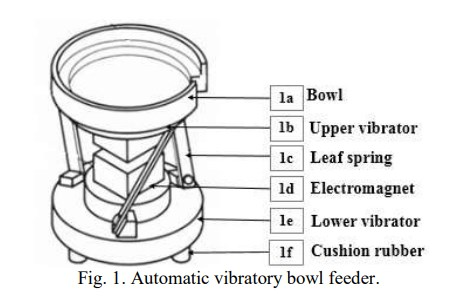
\includegraphics[width=\textwidth]{imgs/articles/feeder.jpg}
      \caption{VBF \citet{nam2019design}}
      \label{fig:feeder}
    \end{minipage}
    \hfill
    \begin{minipage}[t]{0.45\textwidth}
        \centering
        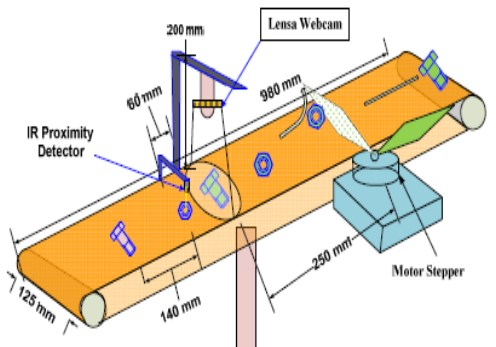
\includegraphics[width=\textwidth]{imgs/articles/conveyer.jpg}
        \caption{Conveyer Belt \citet{Dhenge2013MechanicalNS}}
        \label{fig:conveyer}
        \end{minipage}
\end{figure*}

\section{Background}
For the background of this project, it is necessary to consider literature related to the following:
\begin{mylist}
  \item Mechanical design of existing sorting machines
  \item Existing Computer Vision systems for component identification
  \item Real-time Computer Vision architectures
\end{mylist}
\subsection{Mechanical Design}
\noindent
\textbf{Bowl Feeders} \\
In my research, I have discovered that most industrial sorting machines use a Vibratory Bowl Feeder (VBF) to feed components into the system;
as shown in Figure \ref*{fig:feeder}, the VBF consists of a bowl that vibrates coupled with a spring and electromagnet to feed components into the system.
The paper by \citet{nam2019design} explores the optimal design of a VBF for USB keycaps, by attempting to identify the ideal parameters for the structure of the bowl,
sorting track, mounting adapter, and suspension system. The paper also uses modal analysis to determine the natural frequencies of the system, and uses this to
avoid resonant conditions that might cause inefficient or erratic operation.

This paper is useful as it provides a comprehsive overview of the design of a VBF, and provides a good starting point for the design of the VBF for in the future
when the project is extended to include a VBF for fully autonomous sorting. The paper also provides a good overview of the design considerations for the VBF, and so can be used as a reference
during the design process.

Additionally, \citet{REINHART2010191} delves into the mathematical modelling of a VBF, focusing more on the overall performance of the VBF rather than efficiency, and \citet{ForceAnalysisofVibratoryBowlFeeder}
provides a good overview of the forces involved in the operation of a VBF, stengthening the basis for its design and viability.

The paper by \citet{zhang2019design} outlines a sorting system for vials, and does not make use of a VBF, instead opting for a turntable design that mechanically orientates the vials. It primarily operates
by using a design that is specific to the geometry of the vials, and so is not applicable to this project, however it does provide a good insight into the design of a sorting system.

It seems conclusive that a VBF is the most viable option for the feeding mechanism of the sorting system, and so the design of the VBF will be based on the research outlined above.

\noindent
\textbf{Transport Mechanisms} \\
The paper by \citet{Dhenge2013MechanicalNS} 